\section{Study 2: User Behavior on the TypeBoard}

In this study, we obtained users' typing data on the semi-finished TypeBoard, the touchscreen keyboard developed in study one that prevents unintentional touch. The motivation was to investigate users' typing behavior, based on which we can further improve the TypeBoard.

%we recruited 16 participants and divided them into four groups equally. The first group of participants typed on the existing TypeBoard. After each group finished the experiment, we used the data to improve the TypeBoard. The following participants typed on the improved TypeBoard. That is, we explored the user behavior and improve the method through an iterative process.

\subsection{Participants}

We recruited 16 participants from the local campus (aged from 19 to 37, M = 22.19, SD = 4.55, six females). All the participants were right-handed and did not take part in the first study. They have used software keyboards on smartphones for not less than one year (M = 5.88, SD = 2.36). Ten participants have ever used software keyboards on tablets.

\subsection{Design and Procedure}

As figure \ref{fig:study2_illu} shows, the experimental devices were the same as those in study one, including a Windows Surface tablet computer and a Sensel Morph pressure-sensitive touchpad. The working frequency was 50 FPS. There were text entry tasks, which were the same as study one, namely filling in personal information, short questions, open-book examination, and picture writing. The differences in study two are as follows. First, participants could input words. Second, the keyboard prevented unintentional touch. Intentional touches would trigger keystrokes and audio feedback, while the system ignored unintentional touches.

\begin{figure}[!tbh]
	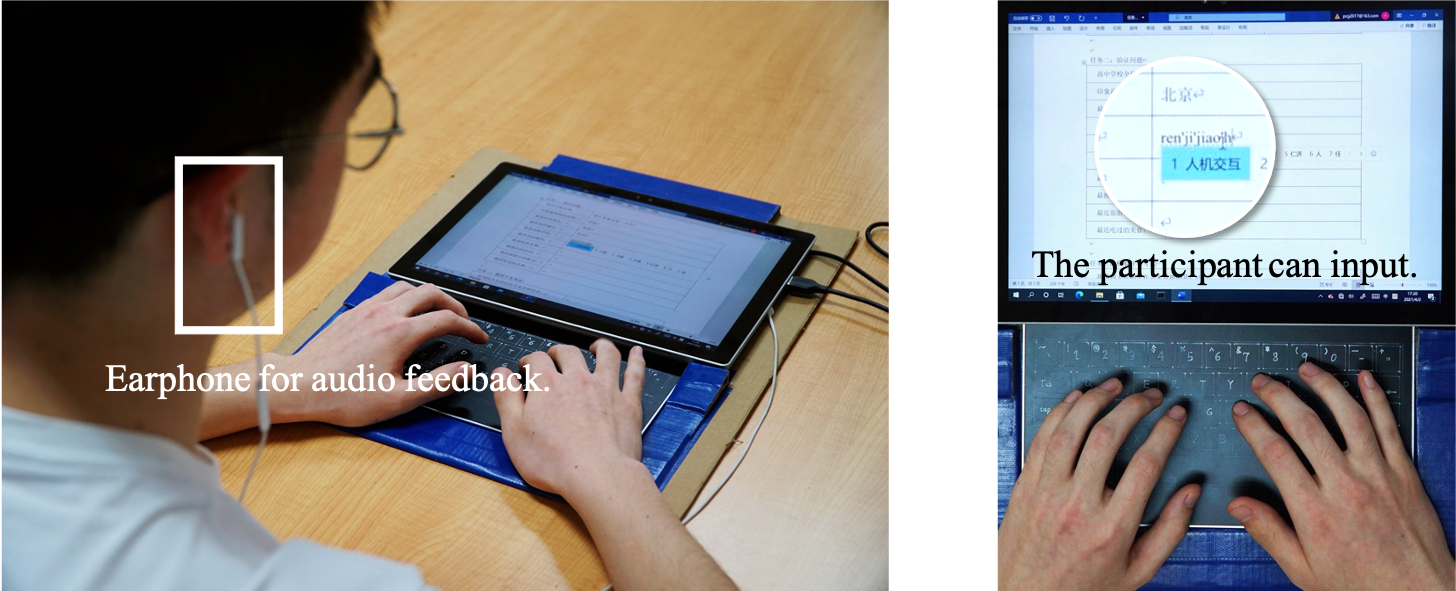
\includegraphics[width=0.9\linewidth]{figures/study2_illu.png}
	\centering
	\caption{The experimental setting of study two.}
	\label{fig:study2_illu}
\end{figure}

Before the experiment, participants warmed up through five-minute free writing. Because no participant had experience typing on a keyboard with unintentional touch prevention, we reminded the participants that they could rest their fingers on the keyboard. Participants could decide to rest their fingers or not according to the task and their preference.
After finishing each task, the participant labeled the data using the label program introduced in study one. During the labeling process, we compared participants' labels with the predictions by the semi-finished TypeBoard. When the two results were different, we recorded the data point for later processing. If the experimenter could not explain the difference, he would discuss it with the participant.
On average, participants spent 10 minutes completing the text entry tasks and spent one hour labeling the data. Participants rested for five minutes between two tasks to avoid fatigue. The study lasted for 90 minutes. The experiment took more time than study one because participants needed to input correct words in this study.

%In a few cases, the system repeatedly gave an incorrect response. For example, a participant (P8) usually rested her left thumb on the screen and triggered false touch. This behavior was not observed in study one, so the system could not identify it correctly. In this situation, we encouraged the participant to keep their behaviors when the system gave an incorrect response. In this situation, participants needed to imagine that the desired words were corrected entered.

%Because the ability of unintentional touch rejection will affect the user behavior, we used an iterative process to improve TypeBoard, and ensured that the participants were typing on the latest version of TypeBoard. We divide the 16 participant into four groups. The first group of participants complete the experiment on the naive TypeBoard introduced in study one. After each group of participants finish their experiment, we improved the algorithm by updating training data and adding features in model. We expected that the TypeBoard algorithm was getting stronger, while the data we collected was getting closer to the natural behaviors of typing on a perfect keyboard.

\subsection{Result}

%在实验的过程中,每四个用户的实验结束之后,我们都会采用新的数据来优化防误触算法,如图xx所示是防误触算法随着完成实验人数的增加的变化,其中每个测试点的数据集包含实验二过程中已经收集到的数据加上实验一的所有数据,评测方法是leave-one-out检测。结果表明,随着实验人数的增加,迭代的TypeBoard和初版TypeBoard的差距在显著拉大。这说明TypeBoard的防误触能力在增强,我们采集到的数据也越来越接近用户在一个完美防误触键盘上的打字行为。【图:初版TypeBoard、迭代TypeBoard随着实验人数增加,准确率的变化】

The dataset contained 13789 touches, excluding the ambiguous touches (0.22\%) in the labeling process. After the double-check of labels, the dataset consisted of 71.01\% positive samples (intentional touches) and 28.99\% negative samples (unintentional touches). The semi-finished TypeBoard predicted the intention of touch with an accuracy of 98.05\% (SD=1.51\%) in study two. There were 0.39\% (SD=0.37\%) false positives and 1.56\% (SD=1.37) false negatives. That is, participants encountered 2.20 unrecognized touchpoints and 0.55 false triggering touchpoints every 100 keystrokes in study two.
The recognition rate of the semi-finished TypeBoard dropped from 99.07\% on the study one dataset to 98.05\% on the study two dataset. It indicates that the user behavior changed in study two, so the model trained on the study one dataset did not work perfectly in study two. Because the user behavior observed in study two was closer to the user’s real usage, it is valuable to investigate the differences in user behaviors between the two studies.

% 实验二共收集了13789个数据点,已经排除了0.22\%的用户无法区分的数据点。在经过了和实验一相同的label确认流程之后,数据集中共包含71.01\%的正例和28.99\%的负例。实验一中总结出来的模型在实验二的测试集下,预测准确率为98.05\%(SD=1.51\%),有0.39\%(SD=0.37\%)的漏报和1.56\%(SD=1.37)的误触发。也就是说,在实验二的实验过程中,用户每有100次有意点击中,平均有0.55次漏报和2.20次的误触点。

Compared with study one, we did not find new cases of unintentional touches in this study. However, the user behavior in study two was different from the last study in details. Table \ref{tab:behavior_difference} shows the examples. First, the user's average pressure of intentional touches in this study was significantly lighter than the last study ($t_{15}=2.78, p<.01$). When typing with feedback, users found that they could type letters without much effort, gradually making the touch lighter. Second, there were more continuous touches in this study ($t_{15}=3.57, p<.005$), where a touch is close to the last touch in both time intervals (< 500 ms) and distance (< 0.5 key widths). This is because participants need to remove incorrect words by continuously pressing the backspace in real typing tasks. Third, the study two dataset contained fewer rollover-typing than the study one ($t_{15}=-6.32, p<.001$). Rollover-typing means the next key is pressed before the previous is released. Participants typed slower in study two because they needed to enter correct words. This slower typing speed correlated with fewer keystrokes typed with rollover \cite{2018-Observations}.

% 显著性分析是否支持该结论,用户点击的力度随着任务顺序而递减?

%Besides, some participants used the right key to select the desired work in the candidate list.

% Table generated by Excel2LaTeX from sheet 'Sheet2'
\begin{table}[htbp]
  \centering
  \caption{The differences of user behavior between the two studies. We use t test to evaluate the significance of the difference. If Levene's test rejects the homoscedasticity of data, we use unequal variances t test instead.}
    \begin{tabular}{|p{5em}|p{15em}|p{4.8em}|p{4.8em}|p{3.5em}|p{4.8em}|}
    \toprule
    \textbf{Measure} & \textbf{Introduction} & \textbf{Study one} & \textbf{Study two} & \textbf{Levene's test} & \textbf{T test} \\
    \toprule
    Touch pressure & The average touch pressure of intentional touches in grams. & 188.39g (SD=64.72) & 124.75g (SD=60.71) & Reject & $t_{15}=2.78$, $p<.01$ \\
    \midrule
    Continous touches & The continous touches as a percentage of all intentional touches. & 4.02\% (SD=1.96\%) & 11.89\% (SD=4.41\%) & Pass  & $t_{15}=3.57$, $p<.005$ \\
    \midrule
    Rollover-Typing & The rollover-typing touches as a percentage of all intentional touches. & 17.60\% (SD=9.34\%) & 7.73\% (SD=5.22\%) & Pass  & $t_{15}=-6.32$, $p<.001$ \\
    \toprule
    \end{tabular}%
  \label{tab:behavior_difference}%
\end{table}%

%\midrule
%Multiple fingers resting & The touches caused by multiple finger resting as a percentage of all unintentional touches. & \multicolumn{1}{r|}{} & \multicolumn{1}{r|}{} & \multicolumn{1}{r|}{} & \multicolumn{1}{r|}{} \\

% The system will classify user touches as either intentional (positive) or unintentional (negative).

As figure \ref{fig:unintentional_touch} shows, we counted the unintentional touches caused by each case of user behavior. The number was counted in touches, e.g., we counted the five fingers resting behavior five times. The three most common unintentional touches were multiple fingers resting (82.90\%), hypothenar eminence touching (7.53\%), and extra light touchpoint (3.21\%). For the unintentional touches illustrated with translucent sub-figures, including (h) one finger resting and (i) extra heavy touchpoint, humans could not identify their intention without contextual information. The machine could hardly judge these cases. Fortunately, their proportion in all unintentional touches was only 1.52\%.
We retrained the model using the study two dataset. Leave one out cross-validation shows that the accuracy increased to 98.88\% (SD=0.73\%), significantly surpassed the semi-finish TypeBoard (F = xx, p < xx). There were 0.66\% (SD=0.58\%) false positives and 0.46\% (SD=0.45\%) false negatives. On average, TypeBoard users will encounter 0.65 unrecognized touchpoints and 0.93 false triggering touchpoints every 100 keystrokes. So far, we have finished the design of the TypeBoard.

\begin{figure}[!tbh]
	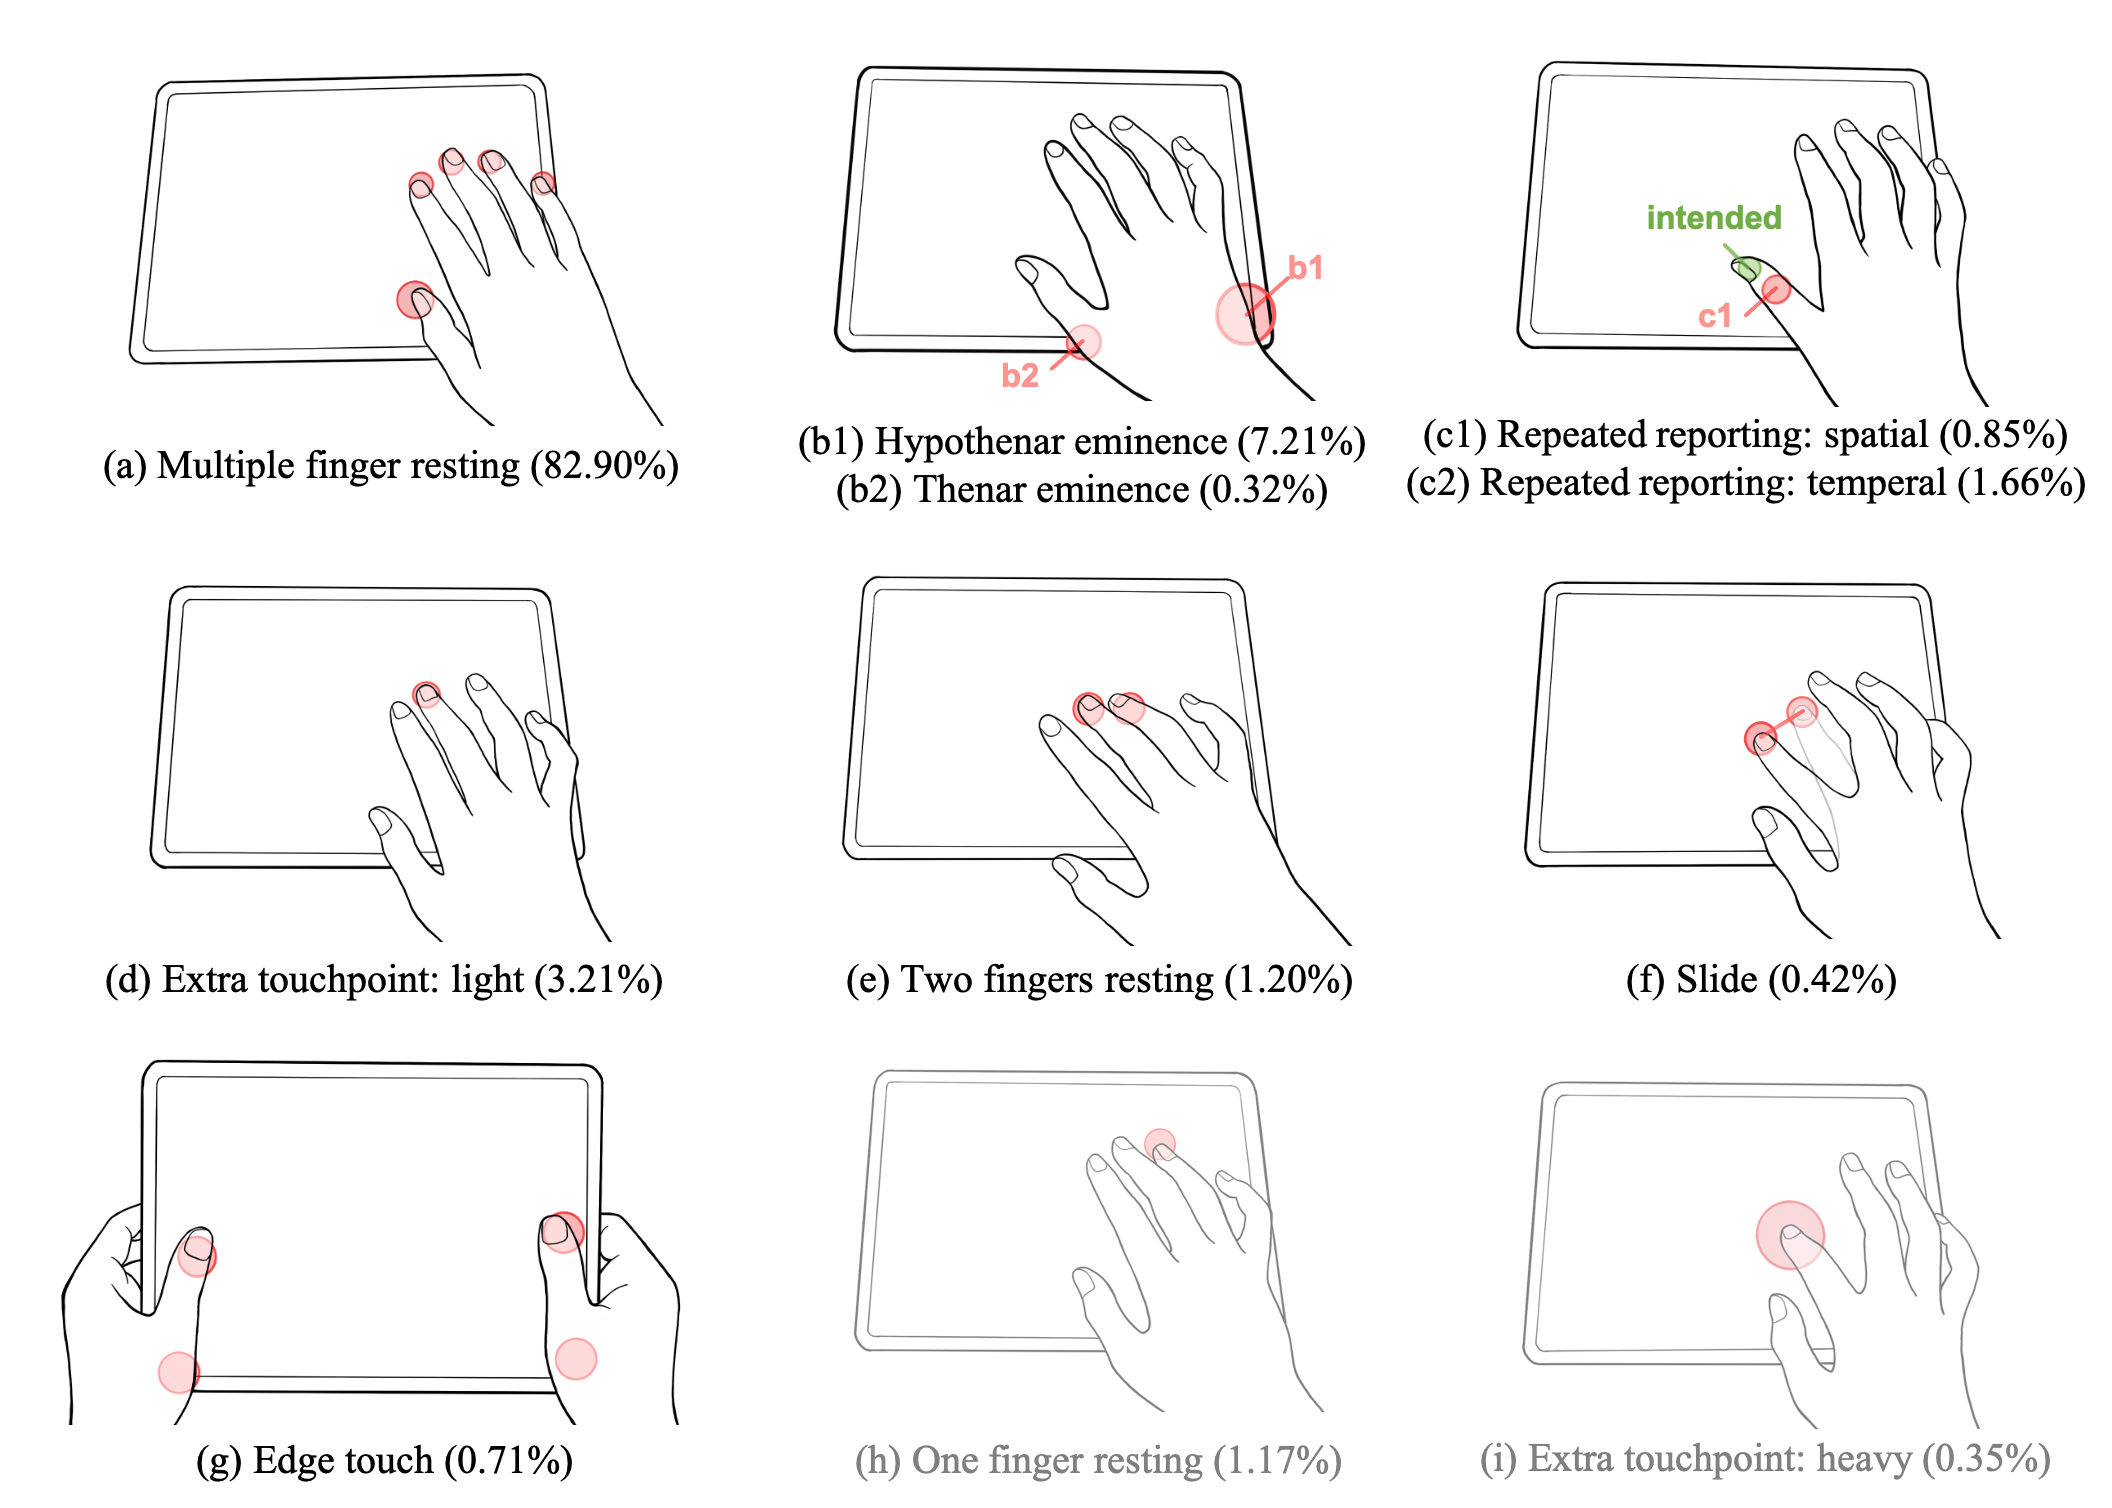
\includegraphics[width=1.0\linewidth]{figures/unintentional_touch.png}
	\centering
	\caption{The classification of unintentional touches. The percentage in the bracket is the proportion of the corresponding cases in all unintentional touches.}
	\label{fig:unintentional_touch}
\end{figure}

%在算法方面,我们也需要将预测算法的训练集替换成实验二所采集到的数据集,重新训练机器学习模型。果然,Leave-one-out验证发现算法的识别准确率提高至98.88\%(SD=0.73\%),且这一提高是显著的(F,p)。

\subsection{Discussion}

\subsubsection{Comparison to previous work}

TapBoard \cite{2013-TapBoard} was the latest study that similar to our work. 
Please note that the TapBoard is different from our proposal TypeBoard. We both investigate unintentional touch prevention on touchscreen keyboards. However, the TapBoard has three defects. First, the TapBoard recognizes "tapping actions" as keystrokes and the others as unintentional touches. Tapping actions were those the duration is shorter than 450 ms, and the displacement is within 15 ms. Users adapt their behavior to meet the technique, which is not natural and relaxing. Second, the TapBoard cannot judge a touch until the touch is released. Even so, the recognition rate is only 97\%. Third, the TapBoard's evaluation was conducted on transcription tasks. The experimental task is not challenging because users seldom rest their fingers on the touchscreen in the transcription task, which was proved in our study three.

We evaluated the TapBoard on our study two dataset, where participants performed natural typing behaviors on the touchscreen keyboard that prevents unintentional touch. The recognition accuracy of the TapBoard was xx.x\% on our dataset, which is nowhere near the performance of our proposal (98.88\%). The result shows that our proposal outperforms existing work.

\subsubsection{The user differences}

As figure \ref{fig:u_touches_over_user_task}(left) shows, the user behaviors of different participants vary a lot. For extreme examples, P1 generated 74.40 unintentional touches every 100 keystrokes, while P16 only produced three unintentional touches during the experiment. We divided participants into three categories. The first type of users (P1-P10) were willing to rest their fingers on the touchscreen. They generated a lot of unintentional touches during the experiment. The second type of users (P11-P12) believed that TypeBoard could prevent unintentional touches. They put their palms on the touchpad but seldom rested their fingers on the keyboard. P12's comment was the key: "\emph{I do not rest my fingers on the touchscreen because I cannot press down directly in the touched state.}" The third type of users (P13-P16) hanged the wrist to input. Surprisingly, they varied a lot in touchscreen keyboard expertise. P13 and P14 had only used touchscreen keyboards for one year, P15 had no experience, while P16 was an expert who performed touch typing on touchscreen keyboards. Results show that personalization is promising to improve the TypeBoard.

\begin{figure}[!tbh]
	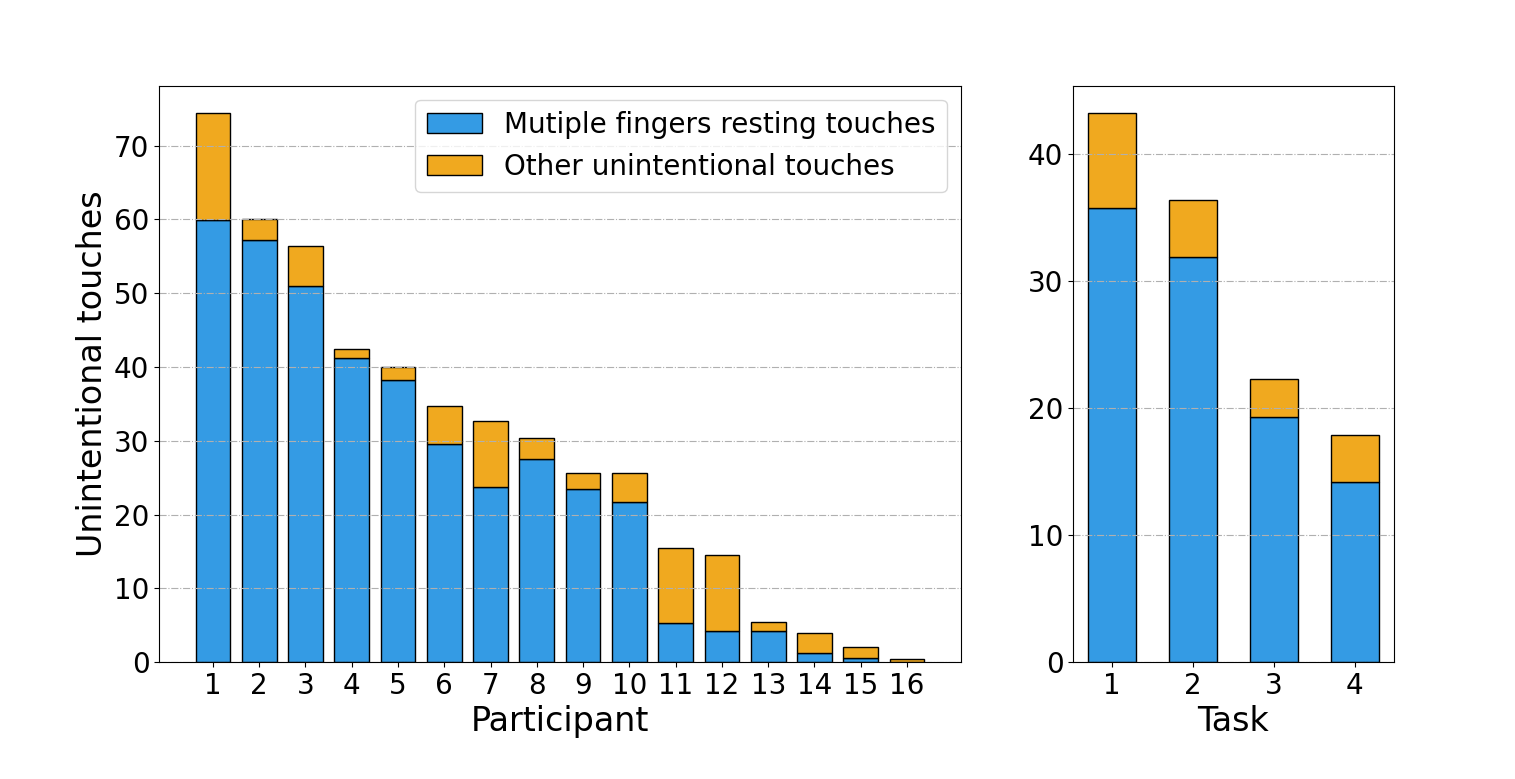
\includegraphics[width=1.0\linewidth]{figures/u_touches_over_user_task.png}
	\centering
	\caption{The unintentional touches per 100 keystrokes over participants and tasks. The blue bars represent those touches that caused by multiple fingers resting, while the orange bars represent other unintentional touches.}
	\label{fig:u_touches_over_user_task}
\end{figure}

\subsubsection{The variety of tasks.}

As figure \ref{fig:u_touches_over_user_task}(right) shows, the task had a significant effect on the number of unintentional touches (F,p). In the four experimental tasks, users produced xx.x (SD=xx.x), xx.x (SD=xx.x), xx.x (SD=xx.x), and xx.x (SD=xx.x) unintentional touches every 100 keystrokes. Bonferroni-corrected post hoc tests showed significant differences between the following task pairs: 1-3 (p<), 1-4 (p<), 2-3 (p<), 2-4 (p<). Users generated more unintentional touches in the first two tasks, which involved more frequent switching between text input and cursor control. Results show that the variety of tasks is important for exploring unintentional touch but usually being neglected in studies \cite{2013-TapBoard, 2020-TabletopTouch, 2014-PalmRejection}.

%The percentages of unintentional touches among the four tasks were 29.73\% (SD=23.71\%), 29.18\%(SD=22.06\%), 18.02\%(18.88\%) and 17.62\%(SD=13.76\%). Bonferroni-corrected post hoc tests showed significant differences between the following task pairs: 1-3 (p<), 1-4 (p<), 2-3 (p<), 2-4 (p<). This result indicates that users generated more unintentional touches on the task with more frequent switching between pointing and typing. We argue that the variety of tasks is important but usually neglected in unintentional touch studies.

\subsection{Why sample five frames in each touch?} 

The more frames we sample in each touch, the more accurate the prediction is. However, a long sampling window means a large delay (20 ms per frame), which affects the user experience. There is a trade-off between the delay and the recognition accuracy. To strike a balance, we simulated our algorithm with different delays. Figure \ref{fig:error_rate_diss}(left) shows the results. An RM ANOVA showed that delay had a significant effect on recognition accuracy ($F_{4,56}=4.88, p<0.05$). Pair-wise comparisons showed significant differences between the following delay pairs: 60-100 (p<.05), 60-120 (p<.05), 60-140 (p<.05), 80-140 (p<.05). Thus, sampling five frames (100 ms) was the best choice, which resulted in acceptable prediction accuracy (98.88\%). Meanwhile, 100 ms is the upper limit of acceptable latency in the touching task \cite{2017-System, 2014-Towards, 2016-Latency}.

\begin{figure}[!tbh]
	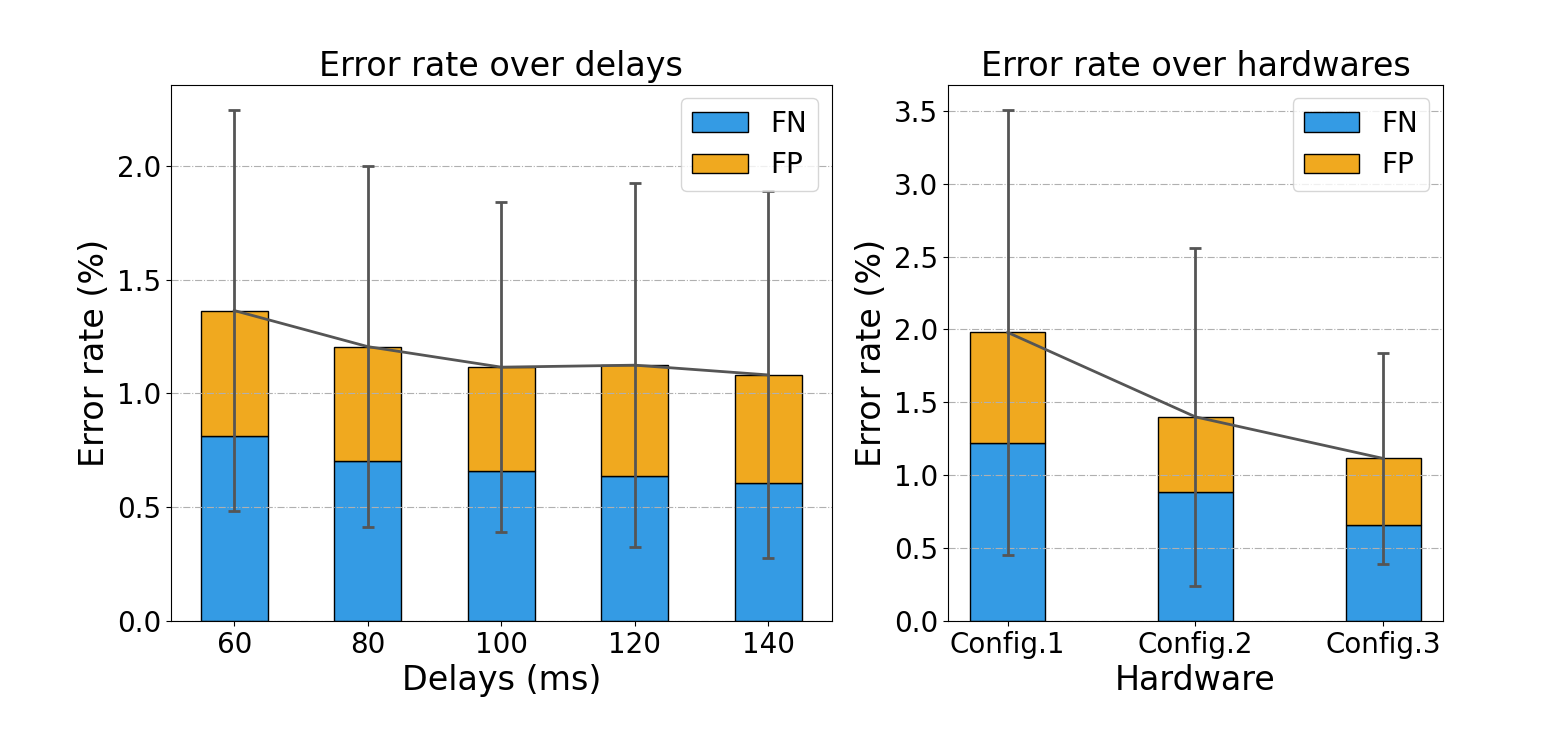
\includegraphics[width=1.0\linewidth]{figures/error_rate_diss.png}
	\centering
	\caption{The recognition error rates over delays and sensor abilities. Error bars indicate standard deviation.}
	\label{fig:error_rate_diss}
\end{figure}

\subsubsection{Can our model work with fewer sensors?}

The pressure signal on the touchscreen is helpful for unintentional touch identification. However, most touchscreen devices have no pressure sensor yet, while a few devices have four pressure sensors in the corners (e.g., the force touch trackpad on MacBook). To explored the feasibility of preventing unintentional touch on existing devices, we evaluated the TypeBoard in three sensor settings. 

\begin{enumerate}
	\item{\textbf{Capactive touchscreen:} The commonly used touchscreen devices have capacitive signals but not pressure signals. To evaluate our method on these devices, we removed all the features referred to pressure signals and retrained the model.}
	\item{\textbf{Force Touch trackpad:} The MacBook's Force Touch trackpad has four pressure sensors in the corners. The trackpad provides the total pressure on the whole touchpad. We evaluated our model in this setting by a simulation, where we estimated the pressure of each touch as the product of the total touchscreen pressure and the contact area proportion of the touch.}
	\item{\textbf{Pressure-sensitive touchscreen:} Future touchscreen devices may provide high-resolution pressure signals, which is the experimental setting in our paper.}
\end{enumerate}

%\item{\textbf{Four pressure signals:} Supposed that we can acquire the four pressure signals in the corners, we are able to calculate the pressure of each touch if there are no more than four fingers on the touchscreen. If there are more than four fingers on the touchscreen, we estimate the pressure as we do in the last condition.}

%现实中大多数触摸屏设备还没有压力传感器,有的设备(如MacBook的force touch trackpad)则在四个角上有压力传感器。为了给防误触触屏提供硬件设计指导,我们对比了我们的算法在三种情况下识别准确率,三种情况分别是:(1)capactive-only:只有电容信号;我们将算法中涉及到压力信号的特征维度都阉割掉来训练机器学习模型。(2)four-force-sensor:四个角上有压力传感器,根据实验采集到的高精度压力信号,我们可以根据基础的物理知识模拟四角压力传感器的数据。我们在情况1的基础上,直接加上四个角压力信号的时域特征。(3)force-enabled:既有电容信号,又有压力信号,这也就是我们论文中所述的配置。

Figure \ref{fig:error_rate_diss}(right) shows our method's performances in the three sensor settings. An RM ANOVA shows a significant effect of setting on the recognition accuracy ($F_{2,28}=10.52, p<0.001$). Bonferroni-corrected post hoc tests showed significant differences between the following setting pairs: 1-2 (p<.005), 1-3 (p<.005). The difference between setting two and three was a tendency (p=.062). Results show that the touchscreen devices with the total pressure signal strike a balance between recognition rate and hardware cost.

%Error rate (SD) / False Positive (SD) / False Negative (SD)
%(1) 0.02028 0.01537 0.01262 0.01212 0.00766 0.00619
%(2) 0.01392 0.01158 0.00876 0.01016 0.00516 0.00542
%(3) 0.01269 0.01175	0.0087 0.01055 0.00399 0.00396
%(4) 0.01115 0.00726 0.00659 0.00578 0.00456 0.00451
